\documentclass[11pt,a4paper]{article}

\usepackage[margin=2.5cm]{geometry}
\usepackage[T1]{fontenc}
\usepackage[utf8]{inputenc}
\usepackage{lmodern}
\usepackage{microtype}
\usepackage{graphicx}
\usepackage{booktabs}
\usepackage{array}
\usepackage{longtable}
\usepackage{enumitem}
\usepackage{hyperref}
\usepackage{float}
\usepackage{amsmath}
\usepackage{caption}
\usepackage[colorlinks=true,
            linkcolor=blue,
            citecolor=blue,
            urlcolor=blue]{hyperref}
% \hypersetup{
%     colorlinks=true,
%     linkcolor=black,
%     urlcolor=blue,
%     citecolor=black
% }
\captionsetup{font=small}
\renewcommand{\arraystretch}{1.15}

% Adjust this if needed
\newcommand{\dbms}{Supabase PostgreSQL}

\title{Project Report -- Phase 1 and Phase 2\\Design, Data Quality, Cleaning, and ETL of the \texttt{APP\_SNAPSHOT} Data Mart}
\author{}
\date{}

\begin{document}
\maketitle

GitHub: \url{https://github.com/quangdangnhat/__DW__googleplaystore__}

\section{Introduction}
This report presents the first two phases of the Google Play Store data warehouse project. Phase 1 focuses on the conceptual and logical design of the data mart. Starting from the reconciled relational schema, we identify the fact of interest, build and edit the attribute tree, define dimensions and measures, derive the Dimensional Fact Model (DFM) schema, and translate the conceptual schema into a logical star schema for ROLAP analysis.

Phase 2 focuses on data management. It documents the population of the reconciled database, the baseline data quality assessment, the cleaning and audit strategy, and the ETL process from the clean/reconciled layer to the data warehouse. The final solution is centered on the fact \texttt{APP\_SNAPSHOT}, implemented as a star schema extended with a weighted bridge table for the many-to-many relationship between app snapshots and \texttt{Genre}.

\section{Data Source and Preliminary Requirement Analysis}

\subsection{Data Source}
The project is based on a Google Play Store dataset containing information about mobile applications published in the store. The data includes both descriptive information about applications and quantitative attributes observed at snapshot level, such as rating, number of reviews, number of installs, price, size, and last update date.

From an analytical point of view, this source is appropriate for multidimensional design because it provides:
\begin{itemize}[leftmargin=1.5em]
    \item descriptive attributes that can be organized into dimensions, such as app, category, app type, content rating, and genre;
    \item numerical attributes that can be analyzed as measures;
    \item a temporal business attribute (\texttt{last\_updated\_date}) supporting time-based analysis;
    \item a non-trivial structural aspect, namely the many-to-many association between snapshots and genres.
\end{itemize}

\subsection{Preliminary Requirement Analysis}
The goal of the data mart is to support exploratory and aggregate analysis of the observed state of applications in the store. In particular, the design is intended to support questions such as:
\begin{itemize}[leftmargin=1.5em]
    \item how ratings, reviews, and installs vary across categories;
    \item how free and paid apps differ in price and popularity;
    \item how content rating is associated with the main numerical indicators;
    \item how application snapshots can be analyzed over time through the update date;
    \item how genre-based analyses can be performed despite the many-to-many relationship with app snapshots.
\end{itemize}

These requirements motivate the choice of a snapshot-oriented fact and a star schema suitable for OLAP-style aggregation and slicing. These requirements also support the Phase 3 visualization story, which investigates whether Google Play Store reach is driven more by perfect ratings or by a combination of good-enough quality, free access, category position, and recent updates.

\section{Reconciled Source Schema and Data-Driven Design Approach}

\subsection{Re-engineering Step}
The original source data was first reorganized into a reconciled relational schema. This re-engineering step makes the source more suitable for subsequent data warehouse design by separating descriptive entities, identifying relationships explicitly, and preparing the data for the data-driven conceptual modeling process.

The reconciled database was implemented in \dbms. This report starts from that reconciled layer and derives the conceptual and logical schemas of the data mart.

\subsection{Schema of the Reconciled Database}
Figure~\ref{fig:reconciled_schema} shows the reconciled relational schema used as input for the data-driven design. The central relation is \texttt{reconciled.app\_snapshot}, which stores the snapshot-level numerical attributes and business descriptors. The descriptive tables \texttt{reconciled.app}, \texttt{reconciled.category}, \texttt{reconciled.app\_type}, and \texttt{reconciled.content\_rating} provide the main candidates for dimensions. Moreover, the association \texttt{reconciled.app\_snapshot\_genre} captures the many-to-many relationship between snapshots and genres, which later motivates the multiple arc in the DFM schema and the bridge table in the logical design.

\begin{figure}[H]
    \centering
    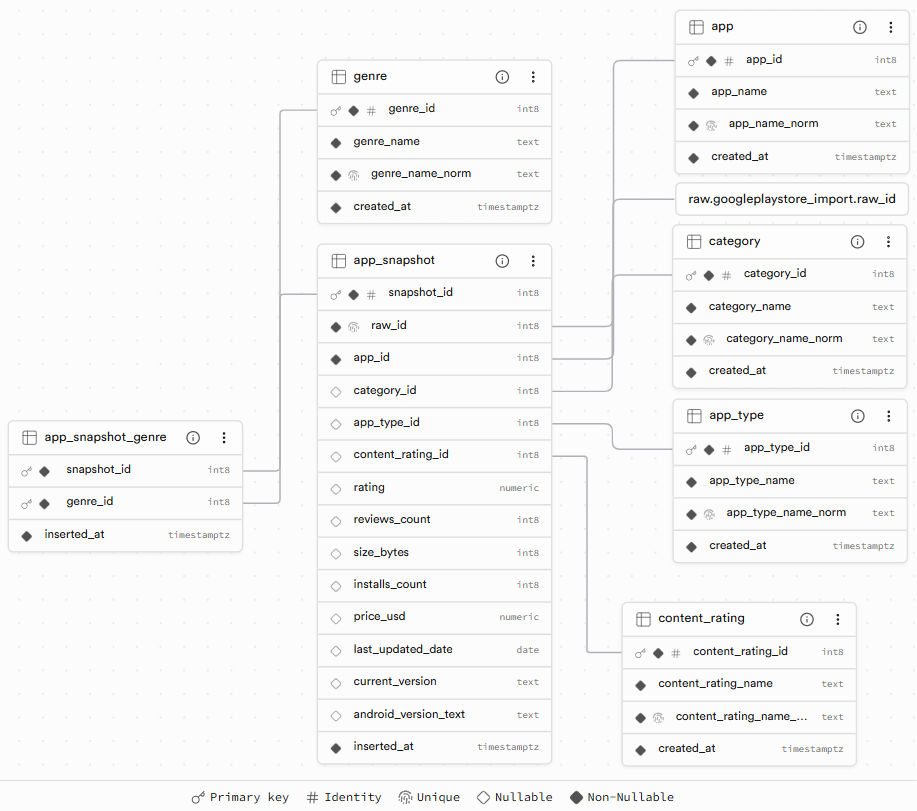
\includegraphics[width=\textwidth]{./figures/reconciledSchema.png}
    \caption{Reconciled relational schema used as input for the data-driven design.}
    \label{fig:reconciled_schema}
\end{figure}

The reconciled schema is implemented in \dbms\ and represents the starting point for the data-driven workflow.

\subsection{Data-driven Design Workflow}
The design follows the data-driven workflow adopted in class:
\begin{enumerate}[leftmargin=1.5em]
    \item definition of the fact;
    \item construction of the basic attribute tree;
    \item editing of the attribute tree;
    \item definition of dimensions;
    \item definition of measures;
    \item design of the final fact schema;
    \item translation into a logical star schema.
\end{enumerate}

\section{Conceptual Design}

\subsection{Definition of the Fact}
The fact chosen for the analysis is \texttt{APP\_SNAPSHOT}. This choice is motivated by the nature of the relation: it represents a dynamic phenomenon of interest for decision-making, namely the observed state of an application at a specific observation point. Each record contains quantitative properties such as rating, number of reviews, number of installs, price, and size, which make the relation suitable for multidimensional analysis.

In contrast, tables such as \texttt{app}, \texttt{category}, \texttt{app\_type}, and \texttt{content\_rating} contain mostly descriptive and relatively stable data, and are therefore more appropriate as dimensions.

At conceptual level, the grain of the fact can be described as one observed snapshot of one application at one update date.

\subsection{Construction of the Basic Attribute Tree}
Starting from the reconciled schema, the basic attribute tree is built by taking the identifier of \texttt{APP\_SNAPSHOT} as the root and recursively following attributes and to-one associations. The resulting tree includes:
\begin{itemize}[leftmargin=1.5em]
    \item direct numerical attributes of \texttt{app\_snapshot}: \texttt{rating}, \texttt{reviews\_count}, \texttt{installs\_count}, \texttt{price\_usd}, \texttt{size\_bytes};
    \item business attributes such as \texttt{last\_updated\_date}, \texttt{current\_version}, and \texttt{android\_version\_text};
    \item to-one related descriptive entities: \texttt{app}, \texttt{category}, \texttt{app\_type}, and \texttt{content\_rating}.
\end{itemize}

The relation \texttt{app\_snapshot\_genre} is not part of the basic attribute tree because it represents a to-many association. Therefore, it does not belong to the basic recursive construction based only on functional dependencies and to-one associations.

\begin{figure}[H]
    \centering
    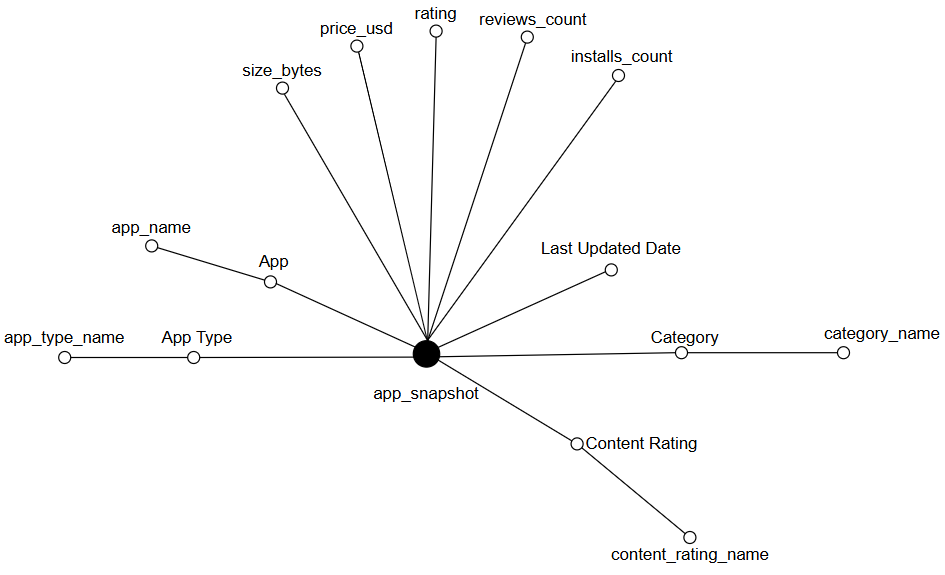
\includegraphics[width=0.9\textwidth]{./figures/attributeTree.png}
    \caption{Basic attribute tree of \texttt{APP\_SNAPSHOT}. The tree includes the direct numerical attributes, the business date \texttt{last\_updated\_date}, and the descriptive entities reachable through to-one associations. The to-many association with \texttt{Genre} is intentionally excluded at this stage.}
    \label{fig:basic_tree}
\end{figure}

\subsection{Editing of the Attribute Tree}
The attribute tree is then edited through pruning and grafting operations.

\paragraph{Pruned elements.}
The following technical attributes are removed because they are not useful for aggregation at the conceptual level:
\begin{itemize}[leftmargin=1.5em]
    \item \texttt{snapshot\_id} in the conceptual representation;
    \item \texttt{raw\_id};
    \item the technical identifiers \texttt{app\_id}, \texttt{category\_id}, \texttt{app\_type\_id}, and \texttt{content\_rating\_id} as labels of intermediate nodes.
\end{itemize}

In addition, \texttt{current\_version} and \texttt{android\_version\_text} are pruned from the conceptual schema because they are not used to define aggregation paths in the current analysis scenario.

\paragraph{Grafted elements.}
The technical identifiers of related tables are replaced by business dimensions and their descriptive leaves:
\begin{itemize}[leftmargin=1.5em]
    \item \texttt{App} $\rightarrow$ \texttt{app\_name}
    \item \texttt{Category} $\rightarrow$ \texttt{category\_name}
    \item \texttt{App Type} $\rightarrow$ \texttt{app\_type\_name}
    \item \texttt{Content Rating} $\rightarrow$ \texttt{content\_rating\_name}
\end{itemize}

\paragraph{Time dimension.}
The business attribute \texttt{last\_updated\_date} is transformed into the temporal dimension \texttt{Date}. The day-level member is the full calendar date, which can be rolled up to month, quarter and year:
\[
\texttt{full\_date} \rightarrow \texttt{month} \rightarrow \texttt{quarter} \rightarrow \texttt{year}
\]
In the logical schema, the attribute \texttt{day} is stored as the day-of-month descriptor of \texttt{full\_date}; it is not interpreted as an independent determinant of month and year. The quarter level is included to support OLAP roll-up and drill-down operations in the Phase 3 dashboards.

\paragraph{Advanced construct.}
The association with \texttt{Genre} is reintroduced at the conceptual level as a multiple arc. This modeling choice is required because the reconciled schema shows that the same app snapshot may be associated with more than one genre.

\subsection{Definition of Dimensions}
After editing the attribute tree, the selected dimensions are:
\begin{itemize}[leftmargin=1.5em]
    \item \texttt{App}
    \item \texttt{Category}
    \item \texttt{App Type}
    \item \texttt{Content Rating}
    \item \texttt{Date}
\end{itemize}

These dimensions determine the granularity of the primary events represented by the fact. The \texttt{Genre} dimension is modeled separately through a multiple arc because its relationship with the fact is many-to-many.

\subsection{Definition of Measures}
The measures are the numerical attributes directly associated with each snapshot:
\begin{itemize}[leftmargin=1.5em]
    \item \texttt{rating}
    \item \texttt{reviews\_count}
    \item \texttt{installs\_count}
    \item \texttt{price\_usd}
    \item \texttt{size\_bytes}
\end{itemize}

From the point of view of additivity, \texttt{rating}, \texttt{price\_usd}, and \texttt{size\_bytes} are treated as non-additive measures. The measures \texttt{reviews\_count} and \texttt{installs\_count} are snapshot-based measures and therefore must be handled carefully along the temporal hierarchy, since summing them across time for the same app may lead to double counting of successive observations.

\subsection{Final DFM Schema}
The final conceptual schema is centered on the fact \texttt{APP\_SNAPSHOT}. The dimensions and hierarchies are:
\begin{itemize}[leftmargin=1.5em]
    \item \texttt{App} $\rightarrow$ \texttt{app\_name}
    \item \texttt{Category} $\rightarrow$ \texttt{category\_name}
    \item \texttt{App Type} $\rightarrow$ \texttt{app\_type\_name}
    \item \texttt{Content Rating} $\rightarrow$ \texttt{content\_rating\_name}
    \item \texttt{Date}: \texttt{full\_date} $\rightarrow$ \texttt{month}  $\rightarrow$ \texttt{quarter} $\rightarrow$ \texttt{year}; the logical attribute \texttt{day} represents the day of month
\end{itemize}

The measures are \texttt{rating}, \texttt{reviews\_count}, \texttt{installs\_count}, \texttt{price\_usd}, and \texttt{size\_bytes}.

The final DFM schema also includes an advanced construct: \texttt{Genre} is represented as a \emph{multiple arc}. This modeling choice is required because the reconciled schema contains the relation \texttt{app\_snapshot\_genre}, and data inspection confirmed that the same snapshot may be associated with more than one genre.

\begin{figure}[H]
    \centering
    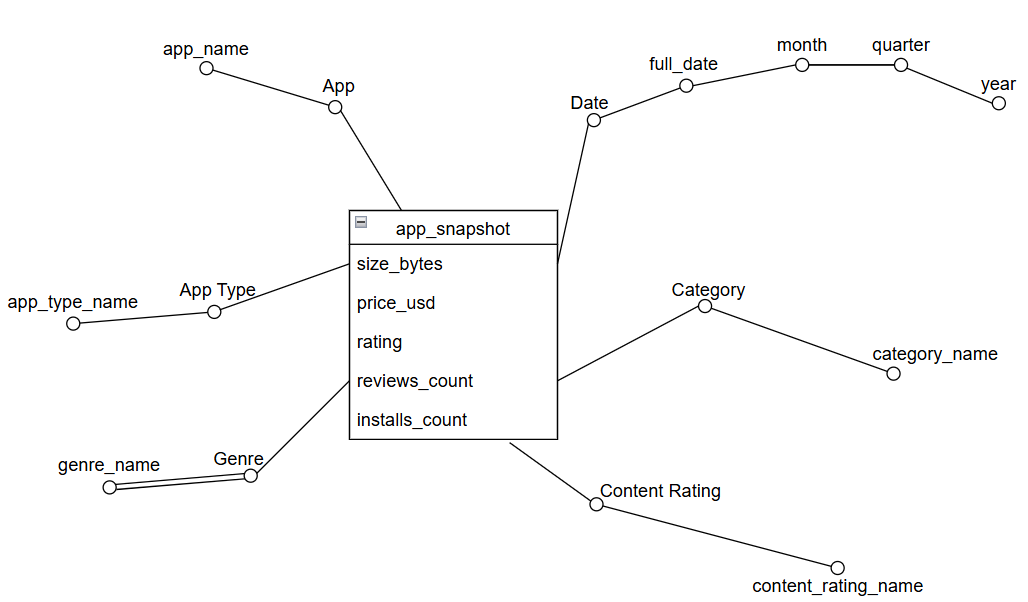
\includegraphics[width=0.92\textwidth]{./figures/DFM_Schema.png}
    \caption{Final DFM schema for \texttt{APP\_SNAPSHOT}. The figure shows the fact, the selected dimensions and hierarchies, and the multiple arc with \texttt{Genre}.}
    \label{fig:dfm_schema}
\end{figure}

\section{Logical Design}

\subsection{Choice of the Logical Model}
The conceptual schema is translated into a ROLAP logical model. The chosen implementation is a star schema. Since the conceptual schema contains a multiple arc involving \texttt{Genre}, the final logical solution is a star schema extended with a bridge table.

The logical schema is also designed for implementation in \dbms.

\subsection{Dimension Tables}
The following dimension tables are created:
\begin{itemize}[leftmargin=1.5em]
    \item \texttt{dim\_app(app\_key, app\_id, app\_name)}
    \item \texttt{dim\_category(category\_key, category\_id, category\_name)}
    \item \texttt{dim\_app\_type(app\_type\_key, app\_type\_id, app\_type\_name)}
    \item \texttt{dim\_content\_rating(content\_rating\_key, content\_rating\_id, content\_rating\_name)}
    \item \texttt{dim\_last\_updated\_date(last\_updated\_date\_key, full\_date, day, month, quarter, year)}
    \item \texttt{dim\_genre(genre\_key, genre\_id, genre\_name)}
\end{itemize}

Each dimension table is identified by a surrogate key and stores the business key coming from the reconciled schema. At logical level, the conceptual dimension \texttt{Date} is implemented through the table \texttt{dim\_last\_updated\_date}, in order to preserve traceability to the source attribute \texttt{last\_updated\_date}.

\subsection{Fact Table}
The fact table is:
\begin{quote}
\texttt{fact\_app\_snapshot(app\_snapshot\_key, snapshot\_id, app\_key, category\_key, app\_type\_key,} \\
\texttt{content\_rating\_key, last\_updated\_date\_key, rating, reviews\_count, installs\_count,} \\
\texttt{price\_usd, size\_bytes)}
\end{quote}

The grain of the fact table is one row for each row of \texttt{reconciled.app\_snapshot}. The attribute \texttt{snapshot\_id} is retained as a business key to preserve traceability with the reconciled layer, while \texttt{app\_snapshot\_key} is the surrogate primary key of the fact table.

\subsection{Bridge Table for the Multiple Arc}

The many-to-many relationship between app snapshots and genres is implemented through the bridge table shown in Figure~\ref{fig:logical_schema}:
\begin{quote}
\texttt{bridge\_app\_snapshot\_genre(app\_snapshot\_key, genre\_key, weight)}
\end{quote}

The primary key of the bridge table is the pair \texttt{(app\_snapshot\_key, genre\_key)}. The attribute \texttt{weight} is used to support weighted analyses over the multiple arc. In the implemented loading workflow, the weight is computed as:
\[
\texttt{weight} = \frac{1}{\texttt{number of genres associated with the snapshot}}
\]

Data checks confirmed that:
\begin{itemize}[leftmargin=1.5em]
    \item the minimum weight is \texttt{0.5};
    \item the maximum weight is \texttt{1.0};
    \item the sum of the weights for each \texttt{app\_snapshot\_key} is equal to \texttt{1}.
\end{itemize}

\subsection{Handling Missing Dimension Values}
During the data management phase, one loaded snapshot was found to have a missing app type in the source data. To preserve the fact grain and avoid nullable foreign keys in the warehouse fact table, the logical loading process introduces a technical \texttt{Unknown} member in \texttt{dim\_app\_type}. This choice does not change the conceptual design; it only affects the ETL strategy and makes the data warehouse robust to incomplete source records. No technical \texttt{Unknown} member was required for \texttt{Content Rating} or \texttt{Date}, because the loaded reconciled snapshots contain valid values for these dimensions.

\subsection{Indexes and Constraints}
The implemented logical schema includes:
\begin{itemize}[leftmargin=1.5em]
    \item primary keys on all dimension tables and on the fact table;
    \item a unique constraint on \texttt{fact\_app\_snapshot.snapshot\_id};
    \item foreign key constraints from the fact table to the dimensions;
    \item a primary key on \texttt{bridge\_app\_snapshot\_genre(app\_snapshot\_key, genre\_key)};
    \item a \texttt{NOT NULL} and \texttt{CHECK} constraint on the bridge attribute \texttt{weight};
    \item indexes on the main foreign keys to improve join performance.
\end{itemize}

\subsection{Glossary of the Measures}
Table~\ref{tab:measure_glossary} provides a glossary of the measures used in the data mart.

\begin{longtable}{@{}p{2.8cm}p{5.2cm}p{2.0cm}p{4.8cm}@{}}
\caption{Glossary of the measures.}
\label{tab:measure_glossary}\\
\toprule
\textbf{Measure} & \textbf{Meaning} & \textbf{Unit} & \textbf{Aggregation behavior} \\
\midrule
\endfirsthead

\toprule
\textbf{Measure} & \textbf{Meaning} & \textbf{Unit} & \textbf{Aggregation behavior} \\
\midrule
\endhead

\bottomrule
\endfoot

\texttt{rating} & Observed average user rating of the app at snapshot time. & score & Non-additive. Typically analyzed through averages rather than sums. \\

\texttt{reviews\_count} & Number of user reviews observed for the app at snapshot time. & count & Snapshot-based. It can be aggregated across non-temporal dimensions, but summing it across time for the same app may double count successive observations. \\

\texttt{installs\_count} & Number of installs observed for the app at snapshot time. & count & Snapshot-based. It can be aggregated across non-temporal dimensions, but summing it across time for the same app may double count successive observations. \\

\texttt{price\_usd} & Observed app price at snapshot time. & USD & Non-additive. Typically analyzed through averages, minima, maxima, or distributions. \\

\texttt{size\_bytes} & Observed app size at snapshot time. & bytes & Non-additive. Typically analyzed through averages, minima, maxima, or distributions. \\
\end{longtable}

\begin{figure}[H]
    \centering
    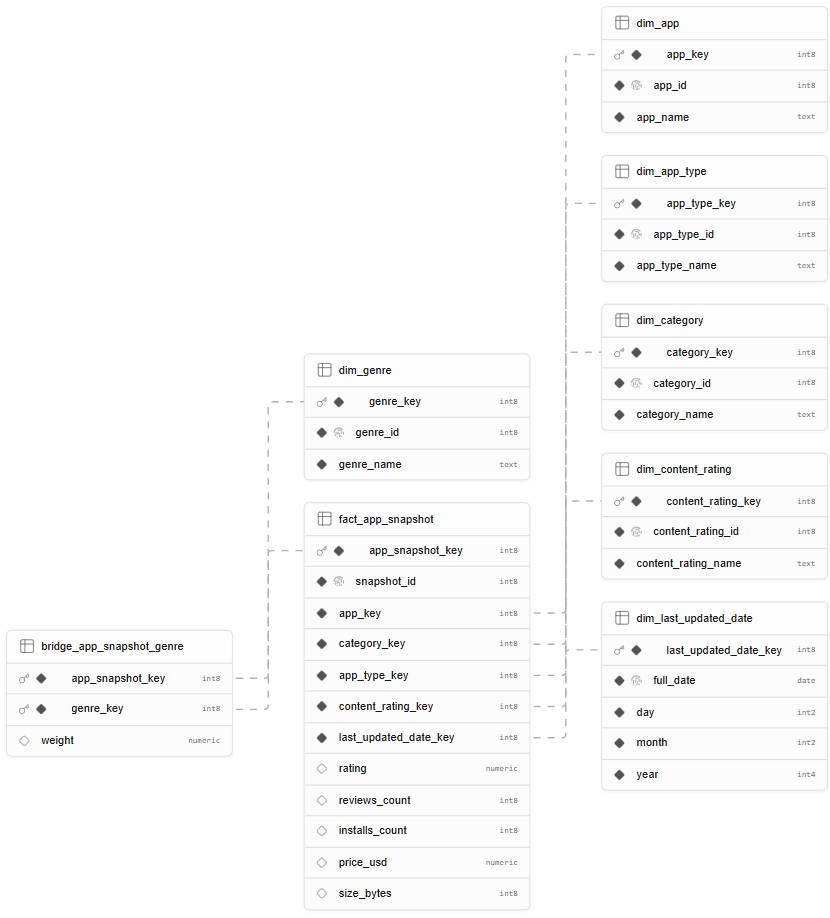
\includegraphics[width=0.9\textwidth]{./figures/starSchema.png}
    \caption{Implemented data warehouse star schema in Supabase PostgreSQL. The schema extends the logical star schema with data quality flags and a weighted bridge table for the many-to-many relationship with Genre.}

    \label{fig:logical_schema}
\end{figure}


\section{Phase 2: Data Management}

\subsection{Objective and Execution Workflow}
The objective of Phase 2 is to populate the reconciled database, assess data quality, implement cleaning tasks, and design the ETL process from the clean/reconciled layer to the data warehouse. The implementation was carried out directly in \dbms\ using SQL scripts. This choice makes the process reproducible, auditable, and close to the final database environment.

The execution order of the implemented scripts is:
\begin{enumerate}[leftmargin=1.5em]
    \item \texttt{01\_reconciled\_schema.sql}: creation of the raw and reconciled schemas;
    \item import of \texttt{googleplaystore.csv} into \texttt{raw.googleplaystore\_import};
    \item \texttt{02\_domain\_load.sql}: loading of domain/master tables;
    \item \texttt{03\_app\_snapshot\_etl.sql}: transformation of raw rows into typed app snapshots;
    \item \texttt{04\_genre\_etl.sql}: extraction of genres and population of the snapshot--genre bridge;
    \item \texttt{05\_dqa\_queries.sql}: baseline data quality assessment;
    \item \texttt{06\_cleaning\_and\_audit.sql}: creation of the clean layer, quality flags, audit log, and weighted genre bridge;
    \item \texttt{07\_dw\_star\_schema.sql}: creation of the data warehouse star schema;
    \item \texttt{08\_dw\_etl.sql}: ETL from the clean layer to the data warehouse.
\end{enumerate}

\subsection{Population of the Reconciled Database}
The original CSV file was first loaded into the raw table \texttt{raw.googleplaystore\_import}. From this raw table, the reconciled schema was populated through SQL transformations. The loading process separates descriptive entities into domain/master tables and stores the numerical snapshot-level attributes in \texttt{reconciled.app\_snapshot}. The many-to-many relationship between snapshots and genres is represented by \texttt{reconciled.app\_snapshot\_genre}.

Table~\ref{tab:phase2_reconciliation_counts} summarizes the reconciliation counts obtained after the raw-to-reconciled loading process.

\begin{table}[H]
\centering
\caption{Reconciliation counts after loading the reconciled database.}
\label{tab:phase2_reconciliation_counts}
\begin{tabular}{@{}lr@{}}
\toprule
\textbf{Metric} & \textbf{Value} \\
\midrule
Raw rows & 10,841 \\
Loaded app snapshots & 10,840 \\
Rows not loaded to snapshot & 1 \\
Apps & 9,638 \\
Categories & 33 \\
App types & 2 \\
Content ratings & 6 \\
Genres & 53 \\
Snapshot--genre bridge rows & 11,288 \\
\bottomrule
\end{tabular}
\end{table}

The single raw row not loaded into \texttt{reconciled.app\_snapshot} corresponds to a shifted malformed source record. It was kept in the raw layer for traceability but excluded from the typed reconciled snapshot table.

\subsection{Baseline Data Quality Assessment}
A baseline data quality assessment was performed on the reconciled layer before cleaning. The checks cover the main operational data quality dimensions used during the course: completeness, uniqueness, validity, consistency, timeliness, and accuracy. Accuracy is documented as a limitation because a trusted external reference source is not available for verifying whether the Google Play Store values reflect real-world truth at the current time.

The most relevant baseline results are shown in Table~\ref{tab:baseline_dqa}. Structural and validity checks are green, while missing ratings and missing/variable sizes are warning-level issues. These warning-level issues are analytically meaningful and therefore should not be blindly imputed.

\begin{table}[H]
\centering
\caption{Selected baseline DQA results on the reconciled layer.}
\label{tab:baseline_dqa}
\begin{tabular}{@{}llrrl@{}}
\toprule
\textbf{Dimension} & \textbf{Metric} & \textbf{Checked} & \textbf{Issues} & \textbf{Severity} \\
\midrule
Completeness & Missing rating & 10,840 & 1,474 & Yellow \\
Completeness & Missing or variable size & 10,840 & 1,695 & Yellow \\
Completeness & Missing app type & 10,840 & 1 & Green \\
Completeness & Missing current version & 10,840 & 8 & Green \\
Completeness & Missing Android version & 10,840 & 2 & Green \\
Uniqueness & Duplicate app normalized name & 9,638 & 0 & Green \\
Uniqueness & Duplicate raw id in snapshot & 10,840 & 0 & Green \\
Uniqueness & Duplicate snapshot--genre pair & 11,288 & 0 & Green \\
Validity & Invalid domain values after load & 41 & 0 & Green \\
Consistency & Type--price conflicts & 10,840 & 0 & Green \\
Timeliness & Missing or future update dates & 10,840 & 0 & Green \\
\bottomrule
\end{tabular}
\end{table}

\subsection{Cleaning Strategy}
The cleaning strategy is conservative. The goal is not to force every missing value to become a value, but to distinguish between data errors and analytically meaningful missing information. For this reason, the pipeline uses the following decisions:
\begin{itemize}[leftmargin=1.5em]
    \item missing ratings are preserved as \texttt{NULL} and marked with \texttt{rating\_missing\_flag};
    \item missing sizes are preserved as \texttt{NULL} and marked with \texttt{size\_missing\_flag};
    \item values equal to \texttt{Varies with device} are explicitly identified by \texttt{size\_varies\_with\_device\_flag};
    \item the single missing app type is preserved and marked with \texttt{app\_type\_missing\_flag};
    \item missing descriptive version attributes are standardized to \texttt{NULL} and flagged;
    \item the many-to-many genre relationship is preserved and handled through a weighted bridge instead of being collapsed to a single genre.
\end{itemize}

This strategy avoids biased imputation of analytical measures such as \texttt{rating} and \texttt{size\_bytes}. It also makes data quality transparent to analysts and dashboard users through explicit flags.

\subsection{Clean Layer and Audit Log}
The script \texttt{06\_cleaning\_and\_audit.sql} creates the schema \texttt{clean}. The main clean tables are \texttt{clean.app\_snapshot\_clean}, \texttt{clean.app\_snapshot\_genre\_clean}, and \texttt{clean.cleaning\_audit\_log}. The clean snapshot table preserves the same grain as the reconciled snapshot table: one row per app snapshot.

Table~\ref{tab:cleaning_summary} reports the main cleaning summary.

\begin{table}[H]
\centering
\caption{Cleaning summary.}
\label{tab:cleaning_summary}
\begin{tabular}{@{}lr@{}}
\toprule
\textbf{Metric} & \textbf{Value} \\
\midrule
Clean app snapshot rows & 10,840 \\
Clean bridge rows & 11,288 \\
Audit log rows & 3,628 \\
Rating missing flag rows & 1,474 \\
Size missing flag rows & 1,695 \\
Size varies with device flag rows & 1,695 \\
App type missing flag rows & 1 \\
Current version missing flag rows & 8 \\
Android version missing flag rows & 2 \\
Type--price conflict flag rows & 0 \\
Invalid measure flag rows & 0 \\
Genre missing flag rows & 0 \\
Multiple genre flag rows & 448 \\
DQ status OK rows & 7,347 \\
DQ status flagged OK rows & 3,493 \\
DQ status error review rows & 0 \\
\bottomrule
\end{tabular}
\end{table}

The audit log records the cleaning or flagging action applied to each affected row. Table~\ref{tab:audit_summary} summarizes the audit log by issue type.

\begin{table}[H]
\centering
\caption{Audit summary by issue type.}
\label{tab:audit_summary}
\begin{tabular}{@{}llr@{}}
\toprule
\textbf{Issue type} & \textbf{Action} & \textbf{Rows} \\
\midrule
\texttt{size\_varies\_with\_device} & \texttt{PRESERVE\_AND\_FLAG} & 1,695 \\
\texttt{rating\_missing} & \texttt{PRESERVE\_AND\_FLAG} & 1,474 \\
\texttt{multiple\_genre\_membership} & \texttt{PRESERVE\_AND\_USE\_WEIGHTED\_BRIDGE} & 448 \\
\texttt{current\_version\_missing} & \texttt{STANDARDIZE\_NULL\_AND\_FLAG} & 8 \\
\texttt{android\_version\_missing} & \texttt{STANDARDIZE\_NULL\_AND\_FLAG} & 2 \\
\texttt{app\_type\_missing} & \texttt{PRESERVE\_AND\_FLAG} & 1 \\
\bottomrule
\end{tabular}
\end{table}

The after-cleaning scorecard confirms that all managed missing values are explicitly flagged, no invalid measures remain, no type--price conflicts are present, no snapshots are missing genres, and the clean row count matches the reconciled row count.

\subsection{Handling the Many-to-Many Relationship with Genre}
The baseline genre distribution confirms that \texttt{Genre} is a real many-to-many analysis dimension. Table~\ref{tab:genre_distribution} shows that 448 snapshots are associated with two genres.

\begin{table}[H]
\centering
\caption{Number of genres per app snapshot.}
\label{tab:genre_distribution}
\begin{tabular}{@{}rr@{}}
\toprule
\textbf{Genre count} & \textbf{Snapshot count} \\
\midrule
1 & 10,392 \\
2 & 448 \\
\bottomrule
\end{tabular}
\end{table}

A direct join between the fact table and the genre bridge would replicate the 448 snapshots with two genres and could lead to double counting. To prevent this issue, \texttt{clean.app\_snapshot\_genre\_clean} computes a bridge weight as:
\[
\texttt{weight} = \frac{1}{\texttt{number of genres associated with the snapshot}}
\]
Thus, a snapshot with one genre receives weight \texttt{1}, while a snapshot with two genres contributes \texttt{0.5} to each genre. The bridge weight check returned zero failing rows, meaning that the sum of weights for each snapshot is equal to \texttt{1}. This directly supports safe OLAP analysis over \texttt{Genre}.

\subsection{Data Warehouse Star Schema Implementation}
The logical star schema designed in Phase 1 was implemented in the schema \texttt{dw}. It contains the following tables:
\begin{itemize}[leftmargin=1.5em]
    \item dimensions: \texttt{dim\_app}, \texttt{dim\_category}, \texttt{dim\_app\_type}, \texttt{dim\_content\_rating}, \texttt{dim\_last\_updated\_date}, \texttt{dim\_genre};
    \item fact: \texttt{fact\_app\_snapshot};
    \item bridge: \texttt{bridge\_app\_snapshot\_genre};
    \item analysis views: \texttt{v\_fact\_app\_snapshot\_enriched}, \texttt{v\_genre\_fractional\_analysis}, \texttt{v\_genre\_membership\_analysis}, and \texttt{v\_genre\_weighted\_kpis}.
\end{itemize}

A technical \texttt{Unknown} member is added to \texttt{dim\_app\_type} to preserve referential integrity for the single snapshot with missing app type. The fact table also includes data quality flags from the clean layer so that dashboard users can filter or explain missing values.

\subsection{ETL from the Clean Layer to the Data Warehouse}
The script \texttt{08\_dw\_etl.sql} populates all dimensions, the fact table, and the genre bridge from the clean and reconciled layers. Table~\ref{tab:dw_load_summary} shows the final data warehouse load summary.

\begin{table}[H]
\centering
\caption{Data warehouse load summary.}
\label{tab:dw_load_summary}
\begin{tabular}{@{}lr@{}}
\toprule
\textbf{Metric} & \textbf{Value} \\
\midrule
\texttt{dim\_app} rows & 9,638 \\
\texttt{dim\_category} rows & 33 \\
\texttt{dim\_app\_type} rows & 3 \\
\texttt{dim\_content\_rating} rows & 6 \\
\texttt{dim\_last\_updated\_date} rows & 1,377 \\
\texttt{dim\_genre} rows & 53 \\
\texttt{fact\_app\_snapshot} rows & 10,840 \\
\texttt{bridge\_app\_snapshot\_genre} rows & 11,288 \\
Unknown app type fact rows & 1 \\
Fact rating missing flag rows & 1,474 \\
Fact size missing flag rows & 1,695 \\
Fact multiple genre flag rows & 448 \\
\bottomrule
\end{tabular}
\end{table}

Integrity checks were executed after the ETL. The results are shown in Table~\ref{tab:dw_integrity_checks}.

\begin{table}[H]
\centering
\caption{Data warehouse integrity checks.}
\label{tab:dw_integrity_checks}
\begin{tabular}{@{}lrrl@{}}
\toprule
\textbf{Check} & \textbf{Expected} & \textbf{Actual} & \textbf{Status} \\
\midrule
Fact rows match clean rows & 10,840 & 10,840 & PASS \\
Bridge rows match clean bridge rows & 11,288 & 11,288 & PASS \\
Genre bridge weight errors & 0 & 0 & PASS \\
Duplicate fact snapshot ids & 0 & 0 & PASS \\
Fact error-review rows & 0 & 0 & PASS \\
\bottomrule
\end{tabular}
\end{table}

The data warehouse therefore preserves the clean-layer grain, maintains referential integrity, and provides safe support for genre-based analyses.

\subsection{Analysis Views for OLAP and BI}
To support correct analysis and reduce the risk of wrong aggregations, several views are created in the data warehouse schema. The most important one is \texttt{dw.v\_genre\_fractional\_analysis}, which exposes weighted measures such as \texttt{weighted\_reviews\_count}, \texttt{weighted\_installs\_count}, and \texttt{weighted\_snapshot\_count}. These fields should be used when aggregating by \texttt{Genre}.

The view \texttt{dw.v\_genre\_membership\_analysis} supports tag-based analysis, where one snapshot may legitimately be counted under more than one genre. In that case, totals across genres are not expected to match the total number of snapshots. This distinction is explicitly documented to prevent double counting in later dashboards. For Phase 3, the main DW analysis views are exported as BI-ready CSV files for Tableau Public, including \texttt{v\_fact\_app\_snapshot\_enriched\_rows.csv} and \texttt{v\_genre\_weighted\_kpis\_rows.csv}. The Tableau genre dashboard uses the exported \texttt{v\_genre\_weighted\_kpis\_rows.csv} file, derived from the weighted genre KPI view, to avoid double-counting multi-genre app snapshots.


\section{Final Result of Phase 1 and Phase 2}
The first two project phases produce the following outputs:
\begin{enumerate}[leftmargin=1.5em]
    \item the identification of \texttt{APP\_SNAPSHOT} as the fact of interest;
    \item the construction and editing of the attribute tree;
    \item the final DFM schema with dimensions, measures, and the multiple arc for \texttt{Genre};
    \item the logical translation into a star schema with a weighted bridge table;
    \item the implementation and population of the raw and reconciled schemas in \dbms;
    \item a baseline data quality assessment on the reconciled layer;
    \item a conservative cleaning strategy based on preservation, explicit flags, and audit logging;
    \item a clean layer preserving the same fact grain as the reconciled snapshot table;
    \item the implementation of the data warehouse star schema;
    \item the ETL process from the clean/reconciled layer to the data warehouse;
    \item integrity checks confirming that fact rows, bridge rows, and genre weights are correct.
\end{enumerate}

\section{Conclusion}
The design and data management phases of the Google Play Store data mart are complete. The conceptual design follows the data-driven DFM methodology, and the logical design translates the model into a relational star schema suitable for OLAP analysis. The implemented data warehouse is centered on \texttt{APP\_SNAPSHOT} and is extended with a weighted bridge table to handle the many-to-many relationship with \texttt{Genre}.

The Phase 2 pipeline confirms that the reconciled database is populated, quality issues are identified, meaningful missing values are preserved and flagged, and all cleaning decisions are recorded in an audit log. The ETL process loads 10,840 cleaned app snapshots into the fact table and 11,288 snapshot--genre associations into the bridge table. All integrity checks pass, including the check that the sum of genre bridge weights is equal to 1 for every snapshot. The resulting warehouse is therefore ready to support the visualization and OLAP analysis activities of Phase 3.

\end{document}